\chapter{不一致ASP程序调试模型的设计}
\label{chp:debug}
在定义了ASP程序的解释模型后,本节将基于该解释模型,进一步定义ASP程序的调试模型。考虑ASP程序的调试场景,大致可以分为两种不同的情况:
\begin{enumerate}[topsep=0pt]
    \setlength\itemsep{-0.3em}
    \item 程序是一致的,但用户预期出现(不应出现)的文字未出现(出现)在回答集中;
    \item 程序是不一致的,但没有回答集或回答集为程序中所有的文字\cite{schulz2015characterising}。
\end{enumerate}

现有的研究普遍将调试集中在不一致程序上,对于一致性程序,当回答集非预期时,用户可以通过本文的解释模型查看该文字真值出现的具体原因。因此,本章在设计调试模型时,也将重点放在不一致逻辑程序的模型中。首先介绍静态分析的调试入口推荐,给出推荐算法;进一步基于调试入口设计基于解释空间的不一致程序调试模型,给出模型的定义及其核心交互算法。
\section{基于程序静态分析的调试入口推荐}
对于不一致的ASP程序,其调试的难点通常在于面对\textit{UNSATISFIABLE}的求解结果,即使用户心中已有明确期待的一个或多个回答集文字,程序的问题也不一定出现与这些文字在相关的规则或事实中,也可能是其他部分的矛盾导致了整个回答集都无法获得。当程序规模较大或程序逻辑较为复杂的时候,用户只能试探性地猜测可能出现问题的规则将其从程序中删除,再尝试对剩余部分求解。这样的行为效率较低,并且删除掉的规则未必就是存在问题的规则。因此,亟需在程序编写完成后对其进行一个静态分析,以快速定位导致程序不一致问题的文字,提示用户对包含这些文字(及其关联规则)重点关注,推荐作为调试的入口;另一方面,为了更真实地将命令式语言的调试风格引入ASP程序,考虑设计一个单步调试模型,使得规则间无序的ASP程序在用户的交互下按照交互步有序执行,直到发现程序中的问题。本节介绍基于程序静态分析的调试入口推荐及其算法。
对不一致ASP程序的研究已经有很多丰富的结论,其中Schulz等人对不一致程序给出了三种情形的讨论\cite{schulz2015characterising},全面系统地找到了导致ASP程序不一致的原因。该讨论基于良基模型,并且能够指出程序中造成不一致的“元凶文字集(Culprit Set)”。这一过程可作为ASP程序调试模型中调试前进行的一次静态程序分析,并且该过程不依赖于回答集。根据是否具有良基模型,下面将介绍这三种原因,之后进一步详细讨论造成不一致的具体文字或规则,并基于这三种原因给出基于程序静态分析的调试入口推荐算法。
\subsection{不一致程序的三种情形}
实际上,程序中的“否定”(包括强否定与NAF否定)是造成逻辑程序不一致的根本原因。Gelfond与Lifschitz等人已经证明,如果一个逻辑程序不含这两种否定,该程序在稳定模型语义下一定是一致的\cite{gel91b}。对于存在否定的程序,其不一致原因的产生又可以归因于两种情况:1)回答集是程序中全部的文字;2)程序不存在回答集。通过考察程序的良基模型,这两种情况进一步又可以细分为如下3种情景,下面分别通过例子加以说明。

\subsubsection*{情形1:程序$P$没有良基模型,且程序的唯一回答集是$Lit(P)$}
\begin{example}[程序$P_7$]
    \label{eg:4.1}
    考虑下面的一个不一致程序$P_7$ \label{prg:p7}:
    \begin{center}
        \begin{tabular*}{.8\linewidth}{l @{\extracolsep{\fill}} lll}
            $r_1: p \leftarrow q.$ & $r_2: q \leftarrow r.$ & $r_3: r \leftarrow.$ & $r_4: s \leftarrow.$ \\
            $r_5: u \leftarrow not\ t.$ & $r_6: t \leftarrow not\ u.$ & $r_7: \lnot p \leftarrow.$ & 
        \end{tabular*}
    \end{center}
    
    程序\hyperref[prg:p7]{$P_7$}没有良基模型。假设其存在回答集$S$,由于程序中的三条事实$r_3, r_4, r_7$,可得到$r \in S, s \in S, \lnot p \in S$。进一步根据$r_1, r_2$,得到$q \in S, p \in S$,此时$S$中包含了一对互补文字$p, \lnot p$,根据回答集的定义可以得到,若$P_7$存在回答集,则回答集必须是程序中的所有文字,即$S=Lit(P_7)$。又因为$\forall r \in P_7^{Lit(P_7)}, S'=\{p, \lnot p, q, r, s\} \models r$,且不存在$S'' \subset S'$满足程序$P_7^{Lit(P_7)}$的所有规则,而$S'$依然包含互补文字$p, \lnot p$,因此$Lit(P_7)$就是$P_7^{Lit(P_7)}$的回答集,进一步得到$Lit(P_7)$是$P_7$的回答集。可以看到,NAF文字的负环($r_5, r_6$与$u, t$)在这里并没有直接导致不一致的出现,从上述的推导过程可以看到,这个程序不一致的直接原因是$\lnot p$与$p$分别通过不含NAF的规则被蕴含。
\end{example}

\subsubsection*{情形2:程序$P$没有良基模型,同时没有回答集}
\begin{example}[程序$P_8$]
    \label{eg:4.2}
    考虑下面的一个不一致程序$P_8$ \label{prg:p8}:
    \begin{center}
        \begin{tabular*}{.8\linewidth}{l @{\extracolsep{\fill}} ll}
            $r_1: q \leftarrow not\ r.$ & $r_2: \lnot q \leftarrow \lnot s, not\ p.$ & $r_3: r \leftarrow not\ \lnot t$\\
            $r_4: \lnot s \leftarrow.$ & $r_5: \lnot t \leftarrow.$ &
        \end{tabular*}
    \end{center}
    
    程序\hyperref[prg:p8]{$P_8$}没有良基模型。假设其存在回答集$S$,由于程序中的事实$r_4, r_5$,可得到$\lnot s \in S, \lnot t \in S$。进一步根据$r_1, r_2, r_3$,得到$\lnot q \in S, q \in S$。此时$S$中包含了一对互补文字$q, \lnot q$,根据回答集的定义可以得到,若$P_8$存在回答集,则回答集必须是程序中的所有文字,即$S=Lit(P_8)$。而$P_8^{Lit(P_8)}=\{q \leftarrow ., \lnot s \leftarrow., \lnot t \leftarrow.\}$,该程序的回答集$\{q, \lnot s, \lnot t\}$中不包含互补文字,因此,$Lit(P_8)$不是$P_8$的回答集,这与假设矛盾,程序\hyperref[prg:p8]{$P_8$}没有回答集。与上例不同的是,此处造成不一致的地方虽然也是互补文字($q, \lnot q$),但推出这一对文字的规则中均包含NAF。
\end{example}

因此,上述两种情景中,情景1的不一致归因于其包含的强否定,而情景2的不一致则同时归因于强否定与NAF。事实上,对于没有良基模型的ASP程序$P$而言,有如下定理:

\begin{theorem}
    给定一个回答集程序$P$,若$P$没有良基模型,$\vdash_{MP}$表示命题逻辑推理中的假言推理(modus ponens),推理结论仅使用程序中的$\leftarrow$作为规则得到,则:
    \begin{enumerate}[itemsep=0pt, label=(\arabic*)]
        \item $P$的回答集是$Lit(P)$,当且仅当$\exists a \in HB_P$,使得$P \vdash_{MP} a$且$P \vdash_{MP} \lnot a$,
        \item $P$没有回答集,当且仅当$\nexists a \in HB_P$,使得$P \vdash_{MP} a$且$P \vdash_{MP} \lnot a$。
    \end{enumerate}
\end{theorem}
    注意到例\ref{eg:4.2}中$\lnot q$的推导需要$not\ p$的成立,而$not\ p$是通过“$p$未出现在任何规则头部无法推导”推理得到,因此$P_8 \not\vdash_{MP} \lnot q$,而$P_8 \cup \{not\ p\} \vdash_{MP} a$。本文借用Schulz等人的定义,对于ASP程序$P$及其中的一个文字$a$,若$P \vdash_{MP} a$,则$a$能够被$P$\textbf{严格推出(strictly derivable)};若$P \not\vdash_{MP} a$,但$\exists \Delta\subseteq NANT(P), P \cup \Delta \vdash_{MP} a$,则$a$能够被$P$\textbf{可废止推出(defeasibly derivable)}。例\ref{eg:4.1}中,$\lnot p$被程序$P_7$严格推出,而例\ref{eg:4.1}中,$\lnot q$被程序$P_8$可废止推出。

\subsubsection*{情形3:程序$P$有良基模型,但没有回答集}
\begin{example}[程序$P_9$]
    \label{eg:4.3}
    考虑下面的一个不一致程序$P_9$ \label{prg:p9}:
    \begin{center}
        \begin{tabular*}{.8\linewidth}{l @{\extracolsep{\fill}} ll}
            $r_1: r \leftarrow not\ s.$ & $r_2: q \leftarrow not\ s.$ & $r_3: p \leftarrow not\ r.$\\
            $r_4: s \leftarrow not\ r.$ & $r_5: \lnot q \leftarrow not\ s.$ & $r_6: \lnot p \leftarrow not\ r.$
        \end{tabular*}
    \end{center}
    
    程序\hyperref[prg:p9]{$P_9$}有良基模型$\langle \emptyset, \emptyset \rangle$。该程序没有回答集,假设其存在回答集$S$,观察各规则可以发现,文字$s, r$有且仅有一个会出现在$S$中。若$s \in S$,则$p, \lnot p \in S$;若$r \in S$,则$q, \lnot q \in S$,因此$S$只可能是$Lit(P_9)$。又由于$P_9^{Lit(P_9)}=\emptyset$,因此$P_9^{Lit(P_9)}$的唯一回答集为$\emptyset \subset Lit(P_9)$,$Lit(P_9)$不是$P_9$的回答集,进而得到$P_9$没有回答集。与例\ref{eg:4.2}不同的是,此处导致互补文字出现的虽然仍NAF导致,但NAF成立的条件为程序中的负环($r_1, r_4\ \text{与 }\ s, r$)。
\end{example}

\subsection{基于导致不一致文字集合的调试入口推荐算法}
在上述三种情形的讨论中,已经以非形式化的说明分析了导致三类不同的程序出现不一致的具体文字。与本章开头的结论相一致,两类否定,即强否定与NAF是造成程序不一致的唯一可能原因。下面以定理的方式形式化地给出导致三类程序不一致的文字集合结论,其中第三类程序需要分两种情况讨论,定理的证明见附录。

\begin{theorem}
    \label{thm:incstlit}
    对一个非一致性ASP程序$P$,$P'$通过将$P$中所有的强否定文字$\lnot a$替换为$a'$得到的一个转换程序,$INCST(P)$为直接导致其不一致的文字集合,$\langle WF^+_{P'}, WF^-_{P'} \rangle$则:
    \begin{enumerate}[itemsep=0pt, label=(\arabic*)]
        \item $P$无良基模型,唯一回答集为$Lit(P)$:
        $$INCST(P)=\{a, \lnot a\ \mid (a, a' \in WF^+_{P'}) \land (P' \vdash_{MP} a) \land (P' \vdash_{MP} a')\}$$
        \item $P$无良基模型,无回答集:
        $$INCST(P)=\{a, \lnot a\ \mid a\ \text{或} a' \text{被程序} P' \text{可废止推出}\}$$
        \item $P$有良基模型(无回答集),但$P'$有回答集$S'$:
        $$INCST(P)=\{a, \lnot a\ \mid (a, a' \in S'), a\ \text{或} a' \text{被程序} P' \text{可废止推出}\}$$
        \item $P$有良基模型(无回答集),但$P'$没有回答集$S'$:
        $$INCST(P)=\{b_1, \ldots, b_o, b_1\ \mid (b_1, \ldots, b_o, b_1) \in cyc^-(P), b_i\ \text{不在程序的三值模型中}\}$$
    \end{enumerate}
\end{theorem}

根据上述四个定理,本文对用户输入的程序进行一次静态分析,判断程序不一致落入何种情形,并给出导致其不一致的直接文字集合。进一步,对于不一致程序而言,虽然不存在解释空间(由于没有一致回答集),但可以构建其文字-规则图$ARG$,将包含导致不一致的直接文字集合的最小子图从文字-规则图ARG中提取出来,提示用户需要检查的规则和原子;另一方面,相较于命令式语言的程序,声明式语言程序没有明确的程序入口和执行次序,第三章中的解释模型将“步”的概念引入解释中,因此考虑进一步将其引入调试中,这要求用户指定一个调试的起点(入口),上述定理得到的$INCST$集合可作为用户调试入口的推荐,引导用户从这些文字出发,更快地找到程序的错误。图4-1给出了查找直接导致不一致集合的流程示意图。
\begin{figure}[htbp]
    \centering
    \includegraphics[height=.8\textwidth, valign=c]{figures/不一致集合计算.jpg}
    \caption{不一致集合计算流程示意}
\end{figure}

对于前三种情况,推荐用户直接以$INCST$集合中的文字作为调试起点,并利用下文介绍的调试模型进行调试;对于第四种情况,除了给出$INCST$集合外,还将文字-规则图中的相关奇数负环找出,以供用户在调试前对相关规则进行检查,向用户推荐调试入口的过程如算法\ref{alg:dbgetcrcmd}所示。

\begin{algorithm2e}[H]
    \DontPrintSemicolon
    \SetNoFillComment
    \SetKwInput{Initialization}{初始化}
    \SetKwInput{KwIn}{输入}
    \SetKwInput{KwOut}{输出}
    \setstretch{1.15}
    \caption{获取程序$P$调试的推荐入口}
    \label{alg:dbgetcrcmd}
    \KwIn{不一致ASP程序$P$}
    \KwOut{文字规则结点集合}
    \setcounter{AlgoLine}{0}
    \everypar={\nl}
    $ARG\_P \gets getARG(P)$ \tcp*[l]{获取程序的文字-规则图}
    $negCycles \gets getAllNegCycles(ARG\_P)$ \tcp*[l]{获取原子规则图中的所有负环}
    \tcc{函数c$omputeIncstLitSet$返回程序$P$的不一致情形$incstCond$与导致不一致的集合$incstLit$}
    $incstCond, incstLit \gets computeIncstLitSet(P)$\;
    \eIf {$incstCond \mathrel{\mathtt{!=}} neg\_loop$}{
        \Return $incstLit$
    }
    {
        $subGraph \gets \emptyset$\;
        \ForEach{环$n\_cycle$ 在 $P$所有规则中}{
            \If {$n\_cycle \cap incstLit \neq \emptyset$}{
            $subGraph \gets subGraph \cup n\_cycle$
            }
        }
        \Return $subGraph$
    }
\end{algorithm2e}

下面以第四种情况为例,说明对一个不一致程序$P_{10}$进行静态分析后向用户展示导致不一致的奇数负环并推荐调试入口的过程。

\begin{example}
    考虑程序$P_{10}$,在Clingo下该程序求解结果为“不一致”。该程序描述了经典的会议论文审稿分配问题中的一部分,问题的基本描述如下:会议论文上交后,各会议委员会成员需要给每篇文章一个审稿意愿评分(记为$bid/3$,三个项分别为委员会成员$pc/1$、稿件编号$paper/1$、分数(0,1,2,3))。对每个委员会成员而言,若某文章未被指定意愿评分,该评分默认设置为1分。若一份稿件被某成员指定了评分,则其被定义为$some\_bid/2$,两个项分别为委员会成员$pc/1$、稿件编号$paper/1$。程序$P_{10}$描述了两个成员、一篇文章下的分配问题。
    \begin{align*}
        \label{prg:p10}
        &r_1: some\_bid(M, P) \leftarrow bid(M, P, X). \\
        &r_2: bid(M, P, 1) \leftarrow not\ some\_bid(M, P), pc(M), paper(P).\\
        &r_3: pc(m1;m2).\\
        &r_4: paper(p1).\\
        &r_5: bid(m1,p1,2).
    \end{align*}
    
    从事实部分可以看到,仅有委员会成员$m1$对稿件$p1$指定了意愿为2分,因此$m2$对稿件$p1$的意愿评分应为默认值1分,期待的回答集中应包含$bid(m2, p1, 1)$,然而该程序不一致。该程序存在良基模型$\langle \{pc(m1), pc(m2), paper(p1), some\_bid(m1,p1), bid(m1, p1,\\2)\},\{bid(m2,p1,2), bid(m1, p1, 1)\}\rangle$,由于$P_{10}$中不含显式否定文字,因此$P_{10}'=P_{10}$,转换后的程序依旧没有回答集,根据不一致集合的计算方法,程序的不一致被归为第四种情形,即程序中的负奇数环导致了程序的不一致。该负环为$\{bid(m1, p1, 1), some\_bid(m1,\\ p1), bid(m1, p1, 1)\}$。考察程序$P_{10}$的文字-规则图,同样能看到这一负环,如图\ref{fig:negcyclep10}所示。
    \begin{figure}[!h]
    \centering
    \includegraphics[height=.6\textwidth, valign=c]{figures/pc-incst例子.jpg}
    \caption{$P_{10}$中负环示意}
    \label{fig:negcyclep10}
\end{figure}
    
可以看到,出现问题是由于$bid(m1, p1, 1)$与$some\_bid(m1, p1)$相互依赖导致的,而实际上$some\_bid$谓词的设立是为了标注“被特别指定了评分的稿件”,这其中不应包含1分的情况,否则根据$r_2$默认为未指定评分的文章赋值为1分后,这些未指定评分的文章由于规则$r_1$再次成为$some\_bid$,违背了这一谓词设立的逻辑初衷。在$r_1$体部添加$X \mathrel{\mathtt{!=}} 1$,程序将会产生正确的结果。不过这一部分修改不是本文研究的内容,因此不在此处赘述。
\end{example}

\section{不一致ASP程序的单步调试模型设计}
在给出了不一致程序的调试入口推荐后,本文介绍不一致ASP单步调试模型的设计。图\ref{fig:dbgpycharm}展示了一个广泛使用的现代IDE(PyCharm)对一个Python程序进行调试的界面,界面中的各个窗口和部件已在图中标明。
\begin{figure}[t]
    \centering
    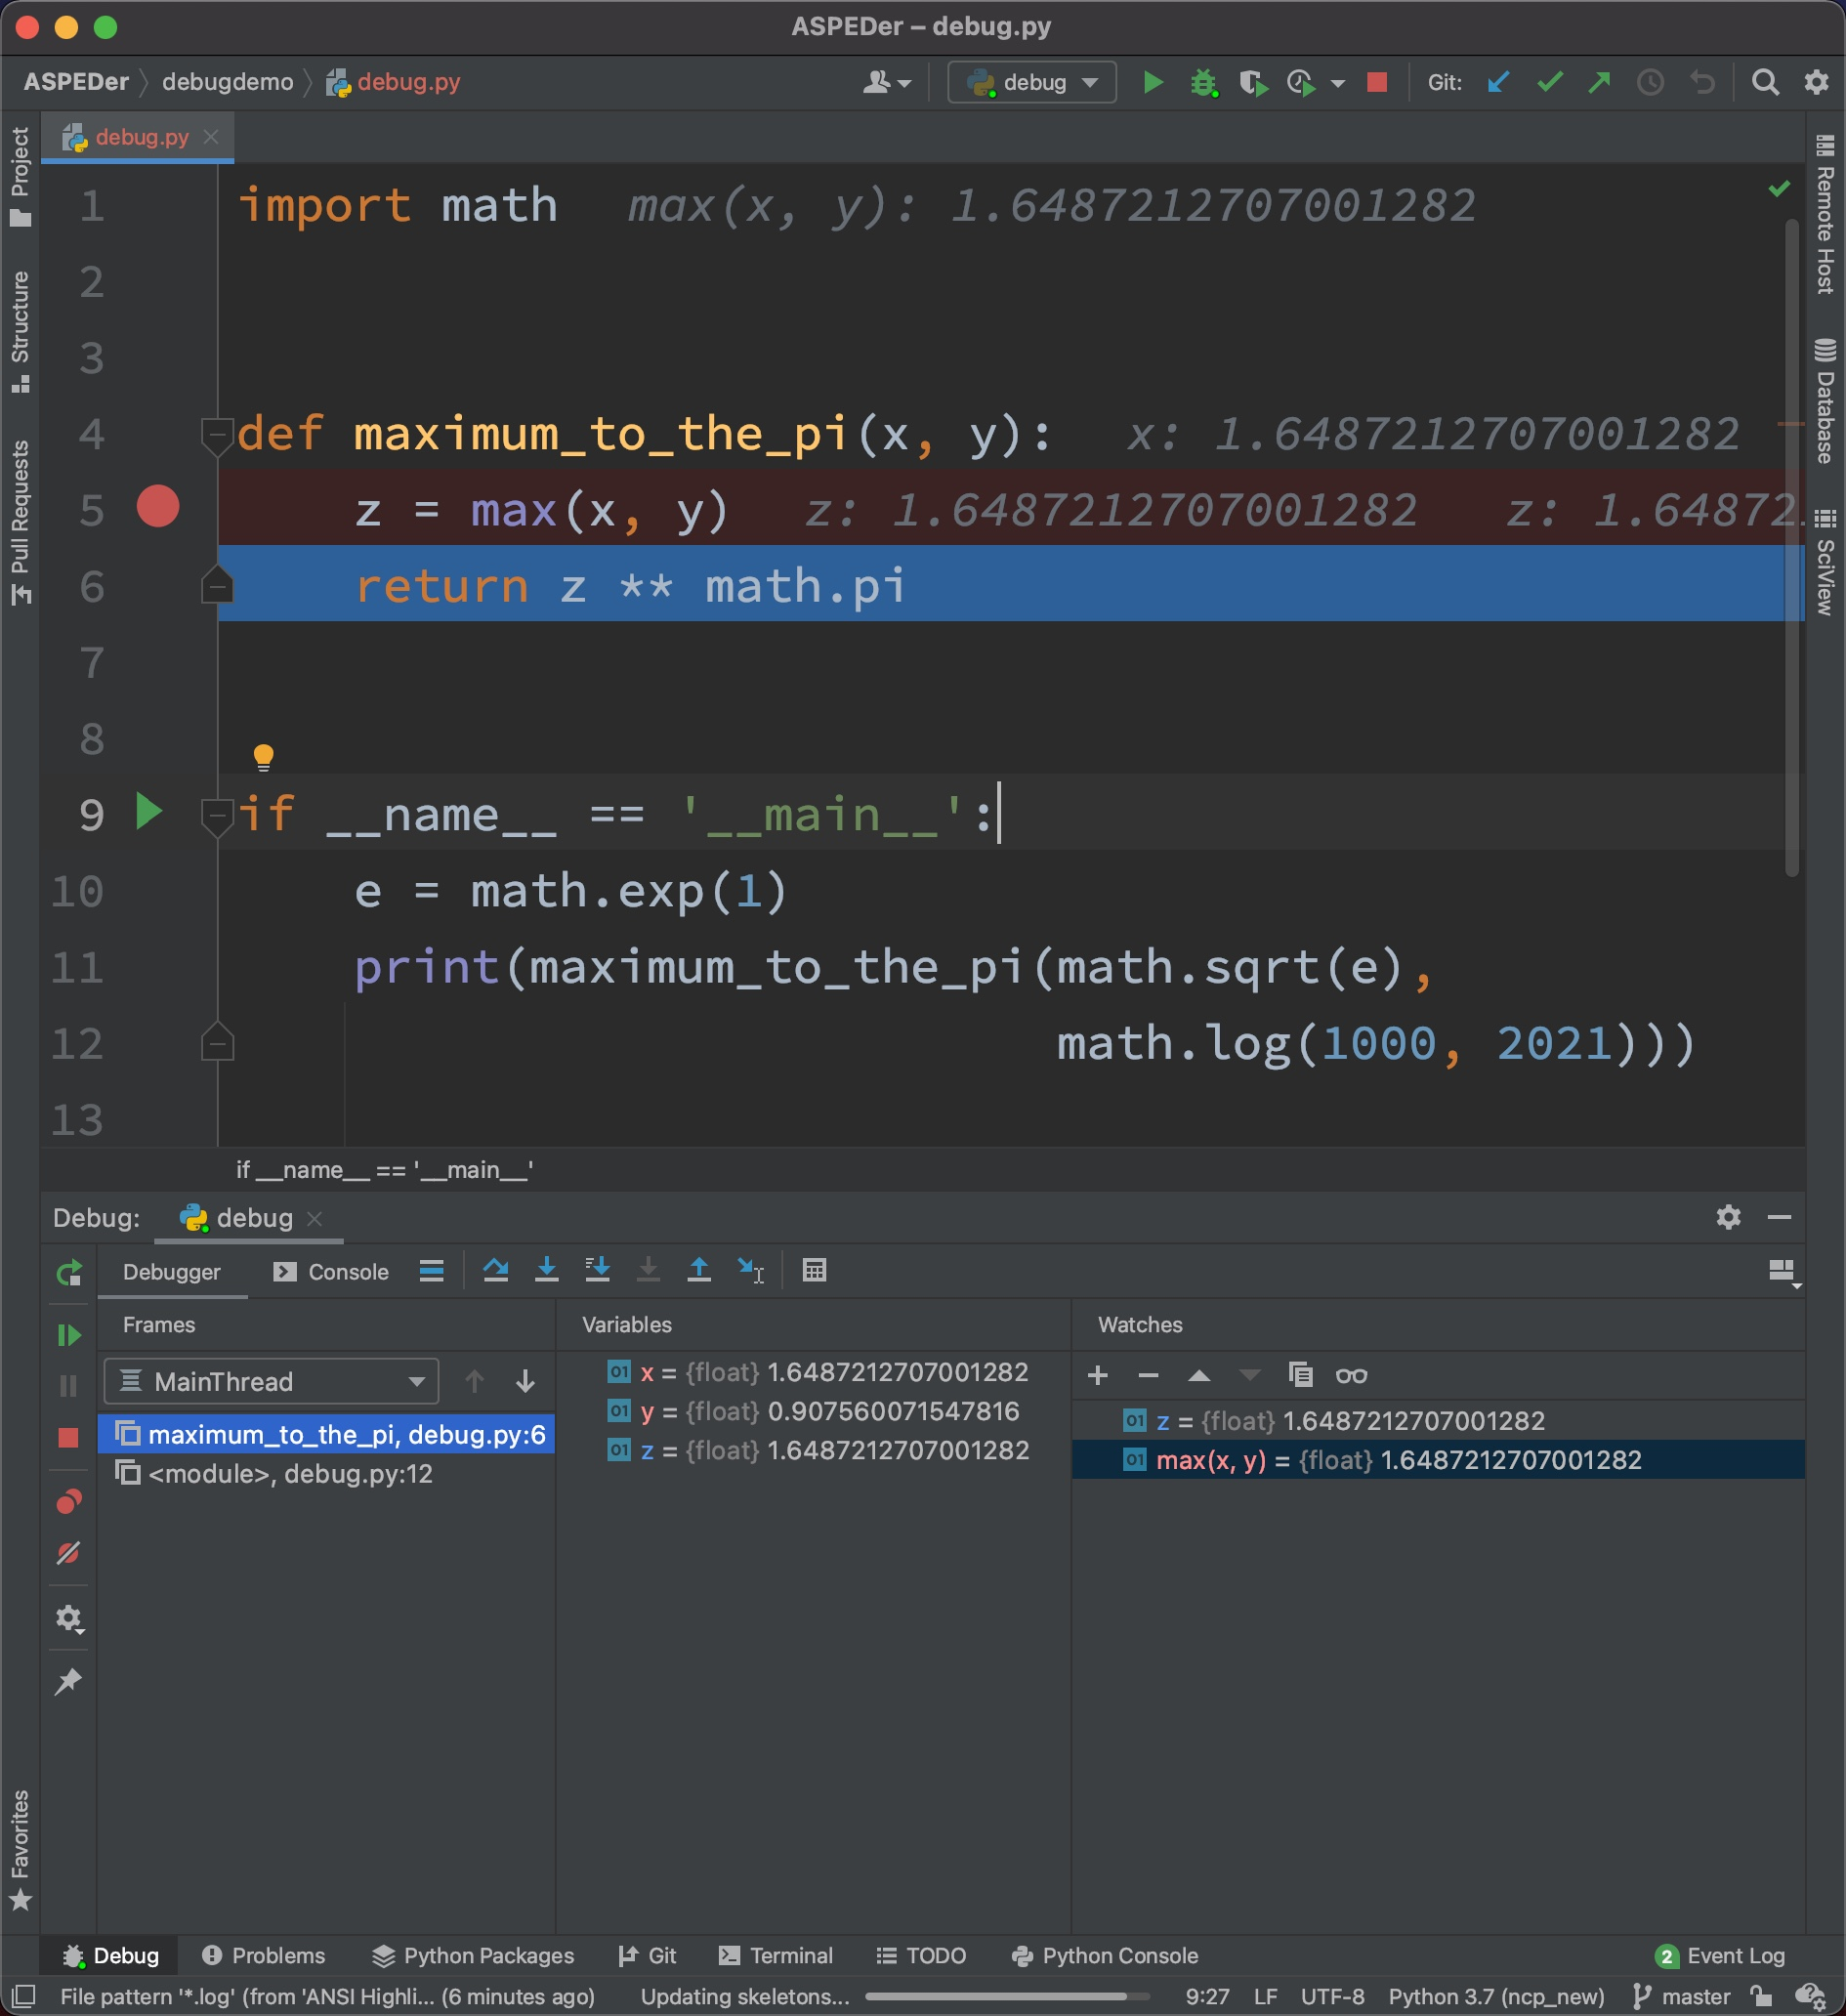
\includegraphics[height=.5\textwidth, valign=c]{figures/现代IDE调试界面.jpg}
    \caption{PyCharm调试某Python程序的界面}
    \label{fig:dbgpycharm}
\end{figure}
可以看到,对于命令式语言,由于存在明确的代码执行次序,因此调试的过程实际上是以主函数main为起点,将程序运行的过程拆解为以代码行为单位的逐条执行过程,用户通过按钮点击驱动程序向下一条执行。本文考虑将这样的调试风格应用于不一致ASP程序的调试中,通过分析ASP程序求解的特性可以发现,直接使用该方法存在两个主要的问题:
\begin{enumerate}[label=(\arabic*), topsep=0pt]
    \setlength\itemsep{-0.3em}
    \item ASP程序没有一个明确的“执行起点”;
    \item ASP程序结论的推导是规则和文字之间交错进行的,没有严格的推导顺序。
\end{enumerate}

虽然ASP程序求解时推导的过程未必严格按照某种顺序进行,但考虑其文字-规则图可以发现,当一个ASP程序确定后,无论其是否为一致性程序、回答集如何,文字-规则图可以唯一确定。进一步,若指定某个文字或规则结点为起点,对该图按照某种策略进行深度优先遍历,则能够确定一条有序的推理路径。这其中,作为起点的“某个文字或规则”,可以通过上一小节所介绍的推荐入口确定,“某种策略”是指在进行深度优先遍历时,当该结点存在多个未访问的邻接结点时,需要由用户指定访问的顺序。

解决了这两个问题后,本文通过类比,将ASP程序调试中的各要素与命令式语言调试的各要素进行一一映射,映射的结果如表\ref{tb:elementmap}所示。

\begin{table}[h!]
    \caption{ASP程序调试与命令式语言调试要素映射表} \label{tb:elementmap}
    \centering
    \renewcommand\arraystretch{2}
    \setlength{\tabcolsep}{15mm}{
    \begin{tabular}{@{}cc@{}}
    \toprule
    命令式程序要素 & ASP程序中的要素 \\ \midrule
    \renewcommand\arraystretch{1.1}
    \begin{tabular}[c]{@{}c@{}}调试的起点函数\\ (用户设置的第一个断点)\end{tabular} & 
    \renewcommand\arraystretch{1.1}
    \begin{tabular}[c]{@{}c@{}}ARG遍历的起点结点\\ (不一致原因集合中用户选择)\end{tabular} \\
    \renewcommand\arraystretch{2}
    当前调试代码语句 & 当前遍历的ARG中的规则结点 \\
    代码中变量的值 & ARG规则结点对应规则中各文字当前真值 \\
    下一步调试的代码语句 & 下一条选中调试的规则 \\ 
    对程序中局部代码的执行 & 对ARG中各依赖边与文字真值的赋值\\
    \bottomrule
    \end{tabular}
    }
    \end{table}

    观察表\ref{tb:elementmap}可以发现,用户调试的过程实际上是在没有回答集或回答集不一致的情况下,通过交互对文字-规则图各结点与边进行标签的赋值,以构建部分解释空间,直到发现矛盾的过程,下面给出不一致ASP程序调试模型的定义。
    \begin{definition}[]
        给定一个不一致ASP程序$P$,其调试模型$Dbg_{incst}(P, l, S, Q, U)$的输入包含如下五个部分:
        \begin{itemize}[topsep=0pt]
            \setlength\itemsep{-0.3em}
            \item 待调试的不一致ASP程序$P$:该程序无变量,回答集为$Lit(P)$或不一致;
            \item 调试的入口文字$l$:满足$l \in INCST(P)$,$INCST(P)$为计算得到的导致不一致的文字集合;
            \item 当前调试步$S$:定义调试中从规则节点到文字节点为一步, 文字节点到规则节点为一步,表示用户当前执行调试进行到的步数;
            \item 退出信号$Q$:表示用户在此步是否选择退出,$Q=t$表示该步骤结束后不继续调试,直接退出; $Q=f$表示该步骤结束后继续调试;
            \item 用户交互信息$U$:用户在交互过程中进行的选择,包含:
            \begin{itemize}[topsep=0pt, label=$\circ$]
                \setlength\itemsep{-0.3em}
                \item 当前步骤位于文字结点,系统无法为该文字标记真值,需要用户根据预期对该文字的真值进行指定;
                \item 当前步骤位于文字结点,该文字结点与多条规则相连接时,用户指定查看某条规则的适用推出/阻塞无法推出的路径;
                \item 当前步骤为规则结点,系统无法确定该规则是否应被适用,需要用户根据预期对该规则的适用情况进行指定;
                \item 当前步骤位于规则结点,该规则结点与多个文字相连接时,用户指定查看规则体部文字的后续推导过程。
            \end{itemize}
        \end{itemize}
    \end{definition}
        
        该模型的输出如式\eqref{eq:dbgincstmodel}所示。
        \begin{equation}
            \label{eq:dbgincstmodel}
            Dbg_{incst}(P, l, s, Q_s, U_s)=
            \begin{cases}
                \text{文字结点} l &s = 0, Q = f\\
                Dbg_{incst}(P, l, s-1, f, \phi) &s > 0, Q = t\\
                Dbg_{incst}(P, l, s-1, f, U_{s-1}) \cup SubExp(P, s, U_s) &s > 0, Q = f\\
                \emptyset &\text{否则}
            \end{cases}
        \end{equation}
    
        与解释模型类似,式\eqref{eq:dbgincstmodel}中仍然是递归定义的,其最核心的部分是$SubExp(P, s, U_s)$的生成,即用户选择进行下一步调试时所呈现的文字-规则子图。其中$U_s$为用户在第$s$步的交互信息,这一信息被定义为一个四元组$U_s=(UL^{true}_s, UL^{false}_s, UR^{ap}_s, UR^{bl}_s)$,为了便于算法的描述,表\ref{tb:usparameter}给出这一四元组的各元素符号表示及含义。
    \begin{table}[H]
        \caption{用户参数$U_s$说明}
        \centering
        \renewcommand\arraystretch{2.5}
        \begin{tabular}{ccc}
        \toprule \noalign{\vspace{-2ex}}
        符号 & 含义 & 取值说明 \\ \hline
        $UL^{true}_s$ & 第$s$步用户指定为真的文字集合 & \multirow{2}{*}{
        \renewcommand\arraystretch{1}    
        \begin{tabular}[c]{@{}c@{}}系统判断该步骤是否可为空,\\ 并给出一个可选文字集合,\\ 若不可为空,则从中选择\\ 一个或多个文字。\end{tabular}} \\
        $UL^{false}_s$ & 第$s$步用户指定为假的文字集合 &  \\ \hline
        $UR^{ap}_s$ & 第$s$步用户指定为适用的规则集合 & \multirow{2}{*}{
        \renewcommand\arraystretch{1}    
        \begin{tabular}[c]{@{}c@{}}系统判断该步骤是否可为空,\\ 并给出一个可选规则集合,\\ 若不可为空,则从中选择\\ 一个或多个规则。\end{tabular}} \\
        $UR^{bl}_s$ & 第$s$步用户指定为阻塞的规则集合 &  \\ \bottomrule
        \end{tabular}
        \label{tb:usparameter}
        \end{table}

    求解这一子图的过程如算法\ref{alg:dbgSubExp}所示。

    \begin{algorithm2e}[H]
        \DontPrintSemicolon
        \SetNoFillComment
        \SetKwInput{Initialization}{初始化}
        \SetKwInput{KwIn}{输入}
        \SetKwInput{KwOut}{输出}
        \SetKwRepeat{Do}{do}{while}
        \setstretch{1.1}
        \caption{程序$P$单步调试子图生成算法}
        \label{alg:dbgSubExp}
        \KwIn{不一致ASP程序$P$,调试步$s$,用户指定的起点文字$l$,用户指定的交互信息$U_s$}
        \KwOut{单步生成的子图}
        \setcounter{AlgoLine}{0}
        \everypar={\nl}
        \While{用户没有停止程序调试}{
        $v_{current} \gets \text{步骤s所位于的结点}$\;
        \eIf {$v_{current} \in V_{Lit}$ \tcp*[l]{当前结点是文字结点}}{
                \If {$v_{current} \not\in (UL_s^{true} \cup UL_s^{false})$ \tcp*[l]{当前文字结点真值尚未被分配}}{
                    \eIf {用户指定$v_{current}$真值为真}{
                        $UL^{true} \gets UL^{true} \cup v_{current}$
                    }{
                        $UL^{false} \gets UL^{false} \cup v_{current}$
                    }
            }

        }
        {
            \If {$v_{current} \not\in (UL_s^{ap} \cup UL_s^{bl})$ \tcp*[l]{当前规则结点规则适用性尚未被分配}}{
                \eIf {用户指定$v_{current}$规则适用}{
                    $UL^{ap} \gets UL^{ap} \cup v_{current}$
                    }{
                        $UL^{bl} \gets UL^{bl} \cup v_{current}$
                    }
            }

        }
        $updateGlobalList(UL^{true},UL^{false},UL^{ap},UL^{bl})$ \tcp*[l]{更新全局文字真值与规则适用性列表}
        }
    \end{algorithm2e}
    
    其中,函数$updateGlobalList$用于在用户一次交互后更新全局为真、为假、规则适用、规则阻塞列表。需要说明,这一函数除了将用户刚刚指定的交互信息添加进入集合,还将根据用户的反馈自动计算能够确定结点的标签,这一计算的过程如算法\ref{alg:updateGlobalList}所示。

    \begin{algorithm2e}[H]
        \DontPrintSemicolon
        \SetNoFillComment
        \SetKwInput{Initialization}{初始化}
        \SetKwInput{KwIn}{输入}
        \SetKwInput{KwOut}{输出}
        \SetKwRepeat{Do}{do}{while}
        \setstretch{1.15}
        \caption{更新全局文字真值与规则适用性列表$updateGlobalList$}
        \label{alg:updateGlobalList}
        \KwIn{不一致ASP程序$P$,当前结点$v_{current}$,全局文字真值与规则适用性列表$U_s=(UL^{true}, UL^{false},UL^{ap})$}
        \KwOut{更新后的全局文字真值与规则适用性列表$U_s$}
        \setcounter{AlgoLine}{0}
        \everypar={\nl}
        \If {$v_{current}$为空}{
            \Return $U_s$
        }
        \If {$v_{current} \in V_{lit}$} {
            $derived\_rules \gets findRuleWithHead(l)$\;
            \If {$v_{current} \in UL^{true}$}{
                \If{$(derived\_rules \cap UL_s^{ap} = \emptyset) \land (||derived\_rules \setminus UL_s^{false}|| = 1)$}{
                    $set\_ap \gets (derived\_rules \setminus UL_s^{false})$\;
                    $UL_s^{ap} \gets UL_s^{ap} \cup set\_ap$
                }
            }
            \If {$v_{current} \in UL^{false}$}{
                $UL_s^{bl} \gets UL_s^{bl} \cup derived\_rules$
            }
            \ForEach{$rule\_node$在$v_{current}$的邻接结点}{
                $updateGlobalList(v_{current}, U_s)$
            }
        }
        \If {$v_{current} \in V_{rule}$} {
            \If {$v_{current} \in UL^{ap}$}{
                $UL_s^{true} \gets UL_s^{true} \cup body^+(v_{current})$\;
                $UL_s^{false} \gets UL_s^{false} \cup body^-(v_{current})$\;
            }
            \If {$v_{current} \in UL^{bl}$}{
                $undecided\_lit \gets body(v_{current}) \setminus (UL_s^{true} \cup UL_s^{false})$\;
                \If{$||undecided\_lit||=1$}{
                    \eIf{$undecided\_lit \cap body^+(v_{current}) \neq \emptyset$}{
                        $UL_s^{true} \gets UL_s^{true} \cup undecided\_lit$\;
                    }{
                        $UL_s^{false} \gets UL_s^{false} \cup undecided\_lit$\;
                    }
                }
            }
            \ForEach{$lit\_node$在$v_{current}$的邻接结点}{
                $updateGlobalList(v_{current}, U_s)$
            }
        }
    \end{algorithm2e}
\section{本章小结}
本章介绍了不一致ASP程序的调试模型。首先介绍并回顾了不一致ASP程序的理论,给出了导致ASP程序不一致的文字集合计算方法,并基于该集合设计了程序调试入口的推荐算法。进一步基于调试入口设计基于解释空间的不一致程序调试模型,重点讨论了在没有回答集及真值的情况下,如何利用解释空间通过调试步骤中的交互,根据用户的反馈引导其发现程序中的错误,最大程度还原了命令式语言的单步调试风格,有效提高了ASP程序的开发效率。